\documentclass[
    % draft,
    fontsize=10pt,
    twoside=off,
    english,
]{scrbook}

\usepackage{scrlayer-scrpage} % Anpassbare Kopf- und Fußzeilen

\usepackage[utf8]{inputenc} % Textkodierung: UTF-8
\usepackage[T1]{fontenc} % Zeichensatzkodierung

%\usepackage[ngerman]{babel} % Deutsche Lokalisierung
\usepackage{graphicx} % Grafiken

% Schriftart Helvetica:
\usepackage[scaled]{helvet}
\renewcommand{\familydefault}{\sfdefault}

% Silbentrennung:
\usepackage{hyphenat}
\hyphenation{TUM in-te-res-siert} % Eigene Silbentrennung
%\tolerance 2414
%\hbadness 2414
%\emergencystretch 1.5em
%\hfuzz 0.3pt
%\widowpenalty=10000     % Hurenkinder
%\clubpenalty=10000      % Schusterjungen
%\vfuzz \hfuzz

\usepackage[hidelinks]{hyperref} % Hyperlinks
\usepackage[onehalfspacing]{setspace} % 1,5facher Zeilenabstand
\usepackage{calc} % Berechnungen
\usepackage{enumitem} % Mehr Kontrolle über itemize-, enumerate- und description-Umgebungen
\usepackage{relsize} % Schriftgröße in Abhängigkeit von aktueller anpassen
\usepackage{tabularx} % Flexiblere Tabellen
\usepackage[tablewithout, figurewithout]{caption} % Anpassen von Beschriftungen

% Nummerierung von Abbildungen & Tabellen durchgängig, statt nach Kapiteln:
%\usepackage{chngcntr}
%\counterwithout{figure}{chapter}
%\counterwithout{table}{chapter}

% Abkürzungen, Glossare:
\usepackage[%
    %xindy,% xindy zum Indexieren verwenden
    acronym,% Separates Akronym-Verzeichnis
    nomain, % CUSTOM
    nopostdot,% Kein Punkt am Ende einer Beschreibung im Glossar
]{glossaries}

% Spezielle Befehlsdefinitionen:
\newcommand{\Thema}{}

\usepackage{amsmath, amsfonts}
	\numberwithin{equation}{chapter}

% B
\usepackage[
    backend=biber,
    style=authoryear,
    sortlocale=de_DE,
    natbib=true,
    url=false, 
    doi=true,
    eprint=false
]{biblatex}
	\addbibresource{refs.bib}
\usepackage{blindtext}
\usepackage{bm}	% bold math >> \boldsymbol command
\usepackage{booktabs}
\usepackage{boxedminipage}
	\setlength{\fboxsep}{5pt}
	\setlength{\fboxrule}{0.1pt}


% C
\usepackage{caption, subcaption} % subfigure
\usepackage{collcell} % \collectcell for custom equation labels in tables
\usepackage{colortbl} % \rowcolor


% E
\usepackage{etoolbox} % booleans: boxes y/n
	\newbool{boxes}
	\booltrue{boxes}
	% \boolfalse{boxes}
    \newbool{api}
    \booltrue{api}
    % \boolfalse{api}


% F
\usepackage{fancybox} % for shaded boxes (ntheorem)
\usepackage{framed} % for framed boxes (ntheorem)

% H
\usepackage{hyperref}

% L
\usepackage{listings}
    \captionsetup[lstlisting]{singlelinecheck=off, font=footnotesize, labelfont=bf}
    \renewcommand{\lstlistingname}{Code} % changes the caption label from Listing to Algorithm
    \renewcommand{\lstlistlistingname}{List of Codes} % changes name of "List of Listings"
    \lstset{
        basicstyle       = \scriptsize\ttfamily,
        breaklines       = true,
        keywordstyle     = \bfseries\color{TUMBlack},
        stringstyle      = \color{JuliaStrings},
        commentstyle     = \color{JuliaComments},
    	backgroundcolor  = \color{CodeBG},
        showstringspaces = false,
    	numbers			 = left,
    	numberstyle		 = \tiny\color{gray},
    	numberbychapter  = false,
    	frame			 = lines,
    	xleftmargin=2em,
    	xrightmargin=0em,
    	framexleftmargin=2em,
    }
	\lstdefinelanguage{Julia}{
        keywordstyle = [2]{\bfseries\color{TUMBlack}},
        %keywordstyle = [3]{\bfseries\color{JuliaTypes}},
        keywordstyle = [3]{\bfseries\color{TUMBlack}},
		%keywordstyle = [4]{\bfseries\color{JuliaBuildIns}},
		keywordstyle = [4]{\bfseries\color{TUMBlack}},
		%keywordstyle = [5]{\bfseries\color{CodeHighlights}},
		keywordstyle = [5]{\bfseries\color{TUMBlack}},
		morekeywords=[2]{ % built-ins
		    abstract,break,case,catch,const,continue,do,else,elseif,
    	  	end,export,false,for,function,immutable,import,importall,if,in,
    	  	macro,module,otherwise,quote,return,switch,true,try,type,typealias,
    	  	using,while,},
		morekeywords=[3]{ % types
			Abstract2DGrid, AbstractMatrix, AbstractVector,
			Bool, 
			Float32, Float64, Function, 
			Int64, Integer, 
			Real, 
			Vector,},
		morekeywords=[4]{pi,@__DIR__,},
		morekeywords=[5]{ % functions
		    CartesianPosition,SphericalPosition,
			lunar_surface_temperatures_BUTLER1997, lunar_surface_temperatures_diviner, lunar_surface_temperatures_diviner_avg, lunar_surface_temperatures_HURLEY2015,
		    mbfluxvdist,
		    rand, range,
			water_vapour_pressure_FRAY2009,},
    	sensitive=true,
    	morecomment=[l]\#,
    	morecomment=[n]{\#=}{=\#},
    	morestring=[s]{"}{"},
    	morestring=[m]{'}{'},
	}[keywords,comments,strings]
	\lstdefinestyle{JuliaAPI}{
		numbers=none,
		framexleftmargin=0em,
    	xleftmargin=0.02\textwidth,
		frame=single,
		linewidth=.98\textwidth,
	}
\usepackage{longtable}



% M
\usepackage{mathtools} % for aligned matrix entries
\usepackage[version=4]{mhchem}
\usepackage{multirow}

% N
\usepackage[skins]{tcolorbox}
\usepackage[framed, hyperref]{ntheorem}
    \theoremstyle{break}
    \def\theoremframecommand{\tcbox[enhanced, sharp corners, drop shadow southeast]}
    \theoreminframepreskip{0cm}
    \theoreminframepostskip{0cm}
    \theoremframepreskip{\topsep}
    \theoremframepostskip{\topsep}
    \theorembodyfont{\footnotesize\itshape}
    \newshadedtheorem{Mybox}{Box}
		\newenvironment{mybox}{\begin{figure}[tb]\begin{Mybox}}{\end{Mybox}\end{figure}}

    \theoremstyle{nonumberplain}
    \theorembodyfont{\footnotesize}
    \newshadedtheorem{Myapi}{API}
		\newenvironment{myapi}{\begin{figure}[tb]\begin{Myapi}}{\end{Myapi}\end{figure}}


% P
\usepackage{pdfpages}
\usepackage{pgf, pgfplots}
	\pgfplotsset{compat=newest}
\usepackage{placeins}

% T
\usepackage{tabu}
\usepackage{tikz}
	\usetikzlibrary{shapes}
	\usetikzlibrary{automata}
	\usetikzlibrary{arrows}
	\usetikzlibrary{backgrounds}
	\usetikzlibrary{calc}
	\usetikzlibrary{positioning}
	\usetikzlibrary{patterns}
	\usetikzlibrary{decorations.pathmorphing}
	\usetikzlibrary{decorations.pathreplacing}
\usepackage{tikz-3dplot}


% S
\usepackage{siunitx}
	\DeclareSIUnit\bar{bar}
	\DeclareSIUnit\LTh{h_{LT}}
\usepackage{subfiles}

% W
\usepackage{wrapfig}
    % \setlength{\wrapoverhang}{15mm}

% X
\usepackage{xcolor}
	%::. TUM colors
	\definecolor{TUMBlack}	    {RGB}{  0,   0,   0}
	\definecolor{TUMGray}	    {RGB}{128, 128, 128}
	\definecolor{TUMGrayDark}   {RGB}{ 51,  51,  51}
	\definecolor{TUMGrayLight}  {RGB}{204, 204, 204}
	\definecolor{TUMWhite}	    {RGB}{255, 255, 255}
	\definecolor{TUMBlue}	    {RGB}{  0, 101, 189}
	\definecolor{TUMBlueDark}   {RGB}{  0,  82, 147}
	\definecolor{TUMBlueDarker} {RGB}{  0,  51,  89}
	\definecolor{TUMBlueLight}  {RGB}{100, 160, 200}
	\definecolor{TUMBlueLighter}{RGB}{152, 198, 234}
	\definecolor{TUMOrange}	    {RGB}{227, 114,  34}
	\definecolor{TUMGreen}	    {RGB}{162, 173,   0}

	%::. Julia colors
	\definecolor{JuliaTypes}{HTML}{397300}
	\definecolor{JuliaBuildIns}{HTML}{78A960}
	\definecolor{JuliaStrings}{HTML}{880000}
	\definecolor{JuliaComments}{HTML}{888888}
	\definecolor{JuliaBlue}{HTML}{4063D8}

	%::.
	\definecolor{CodeBG}{RGB}{245,245,245}
	\definecolor{TableBG}{RGB}{245,245,245}
	\definecolor{CodeHighlights}{rgb}{1.0, 0.55, 0.0}
    \definecolor{NASABlue}{rgb}{0.149, 0.2235, 0.4627}
	\PassOptionsToPackage{table,x11names}{xcolor}

\begin{document}
\renewcommand{\vec}[1]{\boldsymbol{\mathbf{#1}}}

\newcommand{\activationEnergy}{E_a}
\newcommand{\area}{A}
\newcommand{\azimuthAngle}{\alpha}
\newcommand{\baseVector}{\hat{\vec{e}}}
\newcommand{\cartesianCoordinate}{\vec{x}}
    \newcommand{\cartesianCoordinateX}{x}
    \newcommand{\cartesianCoordinateY}{y}
    \newcommand{\cartesianCoordinateZ}{z}
    \newcommand{\cartesianCoordinateDef}{\left[\cartesianCoordinateX, \cartesianCoordinateY, \cartesianCoordinateZ\right]^T}
    \newcommand{\cartesianBaseVectorX}{\baseVector_\cartesianCoordinateX}
    \newcommand{\cartesianBaseVectorY}{\baseVector_\cartesianCoordinateY}
    \newcommand{\cartesianBaseVectorZ}{\baseVector_\cartesianCoordinateZ}
\newcommand{\density}{\rho}
\newcommand{\distance}{d}
\newcommand{\eccentricity}{e}
\newcommand{\eccentricAnomaly}{E} 
\newcommand{\energy}{E}
    \newcommand{\kineticEnergy}{\energy_{kin}}
    \newcommand{\relativeEnergy}{\epsilon}
    \newcommand{\relativeKineticEnergy}{\relativeEnergy_{kin}}
\newcommand{\error}{e}
\newcommand{\extinctionCoefficient}{E}
\newcommand{\force}{F}
\newcommand{\height}{h}
\newcommand{\latitude}{\Phi}
\newcommand{\localTime}{\Time_\text{LT}}
\newcommand{\longitude}{\Theta}
\newcommand{\machineAccuracy}{\epsilon}
\newcommand{\mass}{m}
\newcommand{\mean}{\mu}
    \newcommand{\meanof}[1]{\langle #1 \rangle}
\newcommand{\meanAnomaly}{M}
\newcommand{\numberDensity}{n}
    \newcommand{\surfaceNumberDensity}{n_0}
\newcommand{\partitionFunction}{\zeta}
\newcommand{\period}{P}
\newcommand{\poissonRatio}{\nu}
\newcommand{\porosity}{\Psi}
\newcommand{\potential}{U}
\newcommand{\pressure}{p}
\newcommand{\radius}{r}
\newcommand{\residenceTime}{\tau}
\newcommand{\semiLatusRectum}{p}
\newcommand{\semiMajorAxis}{a}
\newcommand{\sphericalCoordinate}{\vec{r}}
    \newcommand{\sphericalCoordinateRadius}{r}
    \newcommand{\sphericalCoordinateAzimuth}{\vartheta}
    \newcommand{\sphericalCoordinateElevation}{\varphi}
    \newcommand{\sphericalCoordinateDef}{\left[\sphericalCoordinateRadius, \sphericalCoordinateAzimuth, \sphericalCoordinateElevation\right]^T}
    \newcommand{\sphericalBaseVectorRadius}{\baseVector_\sphericalCoordinateRadius}
    \newcommand{\sphericalBaseVectorAzimuth}{\baseVector_\sphericalCoordinateAzimuth}
    \newcommand{\sphericalBaseVectorElevation}{\baseVector_\sphericalCoordinateElevation}
\newcommand{\standardDeviation}{\sigma}
\newcommand{\sublimationFlux}{\Phi}
\newcommand{\temperature}{T}
\newcommand{\thermalAccommodationCoefficient}{\alpha}
\newcommand{\thermalConductivity}{\lambda}
\newcommand{\Time}{t}
    \newcommand{\flightTime}{\Time_{flight}}
\newcommand{\trueAnomaly}{\theta}
\newcommand{\variance}{\standardDeviation^2}
\newcommand{\velocity}{v}
    \newcommand{\Velocity}{V}
\newcommand{\volume}{V}
\newcommand{\youngsModulus}{Y}
\newcommand{\zenithAngle}{\psi}

\hypertarget{meta-title}{%
\section{The Moon}\label{meta-title}}

\begin{center}\rule{0.5\linewidth}{0.5pt}\end{center}

Some introduction text\ldots{}

\hypertarget{lunar-surface-temperatures}{%
\subsection{Lunar Surface
Temperatures}\label{lunar-surface-temperatures}}

Aboard the \(\mathrm{LRO}\) the \(\mathrm{DLRE}\) gathered infrared data
of the lunar surface to create temperatures maps of the Moon.

\section{Figure}

\begin{figure}

\begin{minipage}[t]{0.50\linewidth}

{\centering 

\raisebox{-\height}{

\includegraphics{../../img/documentation/fundamentals/planetary_bodies/moon/lunar_surface_temperatures/lunar_surface_temperature_diviner.png}

}

}

\subcaption{\label{fig-lunar-surface-temperatures-diviner}Based on a
Diviner measurement snapshot.}
\end{minipage}%
%
\begin{minipage}[t]{0.50\linewidth}

{\centering 

\raisebox{-\height}{

\includegraphics{../../img/documentation/fundamentals/planetary_bodies/moon/lunar_surface_temperatures/lunar_surface_temperature_diviner_average.png}

}

}

\subcaption{\label{fig-lunar-surface-temperatures-diviner-average}Based
on the average Diviner measurements.}
\end{minipage}%
\newline
\begin{minipage}[t]{0.50\linewidth}

{\centering 

\raisebox{-\height}{

\includegraphics{../../img/documentation/fundamentals/planetary_bodies/moon/lunar_surface_temperatures/lunar_surface_temperature_BUTLER.png}

}

}

\subcaption{\label{fig-lunar-surface-temperatures-BUTLER}Based on the
analytic function of Butler (1997).}
\end{minipage}%
%
\begin{minipage}[t]{0.50\linewidth}

{\centering 

\raisebox{-\height}{

\includegraphics{../../img/documentation/fundamentals/planetary_bodies/moon/lunar_surface_temperatures/lunar_surface_temperature_HURLEY.png}

}

}

\subcaption{\label{fig-lunar-surface-temperatures-HURLEY}Based on the
analytic function of Hurley et al. (2015)}
\end{minipage}%

\caption{\label{fig-lunar_surface_temperatures}Global, stationary lunar
surface temperature maps. Coordinates given with respect to the subsolar
point at \((\Theta_{ss}, \Phi_{ss}) = (0,0)\), presented in local time
and subsolar latitude.}

\end{figure}

\section{Julia}

\begin{Shaded}
\begin{Highlighting}[]
\ImportTok{using} \BuiltInTok{.ExESS}
\ImportTok{using} \BuiltInTok{CairoMakie}\NormalTok{, }\BuiltInTok{ColorSchemes}
    
\NormalTok{cmap }\OperatorTok{=}\NormalTok{ ColorSchemes.lipari}

\CommentTok{\#::. functions}
\KeywordTok{function} \FunctionTok{\_default\_}\NormalTok{(N}\OperatorTok{=}\FloatTok{240}\NormalTok{, M}\OperatorTok{=}\FloatTok{120}\NormalTok{)}
\NormalTok{    fig     }\OperatorTok{=} \FunctionTok{Figure}\NormalTok{(;resolution}\OperatorTok{=}\NormalTok{(}\FloatTok{600}\NormalTok{,}\FloatTok{285}\NormalTok{))}
\NormalTok{    ga      }\OperatorTok{=} \FunctionTok{MyLTGeoAxis}\NormalTok{(fig[}\FloatTok{1}\NormalTok{,}\FloatTok{1}\NormalTok{];)}
    \FunctionTok{xlims!}\NormalTok{(ga, }\OperatorTok{{-}}\FloatTok{180}\NormalTok{, }\FloatTok{180}\NormalTok{); }\FunctionTok{ylims!}\NormalTok{(ga, }\OperatorTok{{-}}\FloatTok{90}\NormalTok{, }\FloatTok{90}\NormalTok{)}
\NormalTok{    theta   }\OperatorTok{=} \FunctionTok{range}\NormalTok{(}\OperatorTok{{-}}\FloatTok{1}\NormalTok{,}\FloatTok{1}\NormalTok{,N) }\OperatorTok{.*} \ConstantTok{pi} \OperatorTok{.*} \FloatTok{0.995}
\NormalTok{    phi     }\OperatorTok{=} \FunctionTok{range}\NormalTok{(}\OperatorTok{{-}}\FloatTok{1}\NormalTok{,}\FloatTok{1}\NormalTok{,M) }\OperatorTok{.*} \ConstantTok{pi}\OperatorTok{/}\FloatTok{2} \OperatorTok{.*} \FloatTok{0.96}
    \ControlFlowTok{return}\NormalTok{ fig, ga, theta, phi}
\KeywordTok{end}

\KeywordTok{function} \FunctionTok{lunarSurfaceTemperaturesDivinerAverage}\NormalTok{(name}\OperatorTok{=}\StringTok{"lunarSurfaceTemperatureDivinerAverage"}\NormalTok{)}
\NormalTok{    fig, ga, theta, phi }\OperatorTok{=} \FunctionTok{\_default\_}\NormalTok{()}
    
\NormalTok{    N, M }\OperatorTok{=} \FunctionTok{length}\NormalTok{(theta), }\FunctionTok{length}\NormalTok{(phi)}
\NormalTok{    T }\OperatorTok{=} \FunctionTok{lunar\_surface\_temperatures\_diviner\_avg}\NormalTok{(theta, phi)}
\NormalTok{    T }\OperatorTok{=} \FunctionTok{reshape}\NormalTok{(T,N,M)}

\NormalTok{    s }\OperatorTok{=} \FunctionTok{heatmap!}\NormalTok{(ga, }\OperatorTok{{-}}\FloatTok{179}\OperatorTok{..}\FloatTok{179}\NormalTok{, }\OperatorTok{{-}}\FloatTok{89}\OperatorTok{..}\FloatTok{89}\NormalTok{, T; colormap}\OperatorTok{=}\NormalTok{cmap, colorrange}\OperatorTok{=}\NormalTok{(}\FloatTok{50}\NormalTok{,}\FloatTok{400}\NormalTok{))}
\NormalTok{    c }\OperatorTok{=} \FunctionTok{contour!}\NormalTok{(ga, }\OperatorTok{{-}}\FloatTok{179}\OperatorTok{..}\FloatTok{179}\NormalTok{, }\OperatorTok{{-}}\FloatTok{89}\OperatorTok{..}\FloatTok{89}\NormalTok{, T; color}\OperatorTok{=:}\NormalTok{white, levels}\OperatorTok{=}\NormalTok{[}\FloatTok{100}\NormalTok{], linewidth}\OperatorTok{=}\FloatTok{0.7}\NormalTok{)}
\NormalTok{    t }\OperatorTok{=} \FunctionTok{text!}\NormalTok{(ga, }\OperatorTok{{-}}\FloatTok{138}\NormalTok{, }\FloatTok{0}\NormalTok{; text}\OperatorTok{=}\StringTok{"100K"}\NormalTok{, align}\OperatorTok{=}\NormalTok{(}\OperatorTok{:}\NormalTok{center,}\OperatorTok{:}\NormalTok{center), color}\OperatorTok{=:}\NormalTok{white)}

    \FunctionTok{Colorbar}\NormalTok{(fig[}\OperatorTok{:}\NormalTok{,}\FloatTok{2}\NormalTok{], s, label}\OperatorTok{=}\StringTok{"Temperature [K]"}\NormalTok{)}

    \FunctionTok{save}\NormalTok{(}\FunctionTok{joinpath}\NormalTok{(}\PreprocessorTok{@\_\_DIR\_\_}\NormalTok{, }\StringTok{"}\SpecialCharTok{$}\NormalTok{(name)}\StringTok{.pdf"}\NormalTok{), fig)}
    \FunctionTok{save}\NormalTok{(}\FunctionTok{joinpath}\NormalTok{(}\PreprocessorTok{@\_\_DIR\_\_}\NormalTok{, }\StringTok{"}\SpecialCharTok{$}\NormalTok{(name)}\StringTok{.svg"}\NormalTok{), fig)}
    \FunctionTok{save}\NormalTok{(}\FunctionTok{joinpath}\NormalTok{(}\PreprocessorTok{@\_\_DIR\_\_}\NormalTok{, }\StringTok{"}\SpecialCharTok{$}\NormalTok{(name)}\StringTok{.png"}\NormalTok{), fig, px\_per\_unit}\OperatorTok{=}\FloatTok{4}\NormalTok{)}

    \ControlFlowTok{return} \ConstantTok{nothing}
\KeywordTok{end}

\KeywordTok{function} \FunctionTok{lunarSurfaceTemperaturesDiviner}\NormalTok{(name}\OperatorTok{=}\StringTok{"lunarSurfaceTemperatureDiviner"}\NormalTok{)}
\NormalTok{    fig, ga, theta, phi }\OperatorTok{=} \FunctionTok{\_default\_}\NormalTok{(}\FloatTok{720}\NormalTok{, }\FloatTok{360}\NormalTok{)}

\NormalTok{    N, M }\OperatorTok{=} \FunctionTok{length}\NormalTok{(theta), }\FunctionTok{length}\NormalTok{(phi)}
\NormalTok{    T }\OperatorTok{=} \FunctionTok{lunar\_surface\_temperatures\_diviner}\NormalTok{(}\FloatTok{0}\NormalTok{, theta, phi)}
\NormalTok{    T }\OperatorTok{=} \FunctionTok{reshape}\NormalTok{(T,N,M)}

\NormalTok{    s }\OperatorTok{=} \FunctionTok{heatmap!}\NormalTok{(ga, }\OperatorTok{{-}}\FloatTok{179}\OperatorTok{..}\FloatTok{179}\NormalTok{, }\OperatorTok{{-}}\FloatTok{89}\OperatorTok{..}\FloatTok{89}\NormalTok{, T; colormap}\OperatorTok{=}\NormalTok{cmap, colorrange}\OperatorTok{=}\NormalTok{(}\FloatTok{50}\NormalTok{,}\FloatTok{400}\NormalTok{))}
\NormalTok{    c }\OperatorTok{=} \FunctionTok{contour!}\NormalTok{(ga, }\OperatorTok{{-}}\FloatTok{179}\OperatorTok{..}\FloatTok{179}\NormalTok{, }\OperatorTok{{-}}\FloatTok{89}\OperatorTok{..}\FloatTok{89}\NormalTok{, T; color}\OperatorTok{=:}\NormalTok{white, levels}\OperatorTok{=}\NormalTok{[}\FloatTok{100}\NormalTok{], linewidth}\OperatorTok{=}\FloatTok{0.7}\NormalTok{)}
\NormalTok{    t }\OperatorTok{=} \FunctionTok{text!}\NormalTok{(ga, }\OperatorTok{{-}}\FloatTok{138}\NormalTok{, }\FloatTok{0}\NormalTok{; text}\OperatorTok{=}\StringTok{"100K"}\NormalTok{, align}\OperatorTok{=}\NormalTok{(}\OperatorTok{:}\NormalTok{center,}\OperatorTok{:}\NormalTok{center), color}\OperatorTok{=:}\NormalTok{white)}

    \FunctionTok{Colorbar}\NormalTok{(fig[}\OperatorTok{:}\NormalTok{,}\FloatTok{2}\NormalTok{], s, label}\OperatorTok{=}\StringTok{"Temperature [K]"}\NormalTok{) }

    \FunctionTok{save}\NormalTok{(}\FunctionTok{joinpath}\NormalTok{(}\PreprocessorTok{@\_\_DIR\_\_}\NormalTok{, }\StringTok{"}\SpecialCharTok{$}\NormalTok{(name)}\StringTok{.pdf"}\NormalTok{), fig)}
    \FunctionTok{save}\NormalTok{(}\FunctionTok{joinpath}\NormalTok{(}\PreprocessorTok{@\_\_DIR\_\_}\NormalTok{, }\StringTok{"}\SpecialCharTok{$}\NormalTok{(name)}\StringTok{.svg"}\NormalTok{), fig)}
    \FunctionTok{save}\NormalTok{(}\FunctionTok{joinpath}\NormalTok{(}\PreprocessorTok{@\_\_DIR\_\_}\NormalTok{, }\StringTok{"}\SpecialCharTok{$}\NormalTok{(name)}\StringTok{.png"}\NormalTok{), fig, px\_per\_unit}\OperatorTok{=}\FloatTok{4}\NormalTok{)}

    \ControlFlowTok{return} \ConstantTok{nothing}
\KeywordTok{end}

\KeywordTok{function} \FunctionTok{lunarSurfaceTemperaturesBUTLER}\NormalTok{(name}\OperatorTok{=}\StringTok{"lunarSurfaceTemperatureBUTLER"}\NormalTok{)}
\NormalTok{    fig, ga, theta, phi }\OperatorTok{=} \FunctionTok{\_default\_}\NormalTok{()}
\NormalTok{    T }\OperatorTok{=} \FunctionTok{lunar\_surface\_temperatures\_BUTLER1997}\NormalTok{(theta, phi)}
\NormalTok{    s }\OperatorTok{=} \FunctionTok{heatmap!}\NormalTok{(ga, }\OperatorTok{{-}}\FloatTok{179}\OperatorTok{..}\FloatTok{179}\NormalTok{, }\OperatorTok{{-}}\FloatTok{89}\OperatorTok{..}\FloatTok{89}\NormalTok{, T; colormap}\OperatorTok{=}\NormalTok{cmap, colorrange}\OperatorTok{=}\NormalTok{(}\FloatTok{50}\NormalTok{,}\FloatTok{400}\NormalTok{))}

    \FunctionTok{Colorbar}\NormalTok{(fig[}\OperatorTok{:}\NormalTok{,}\FloatTok{2}\NormalTok{], s, label}\OperatorTok{=}\StringTok{"Temperature [K]"}\NormalTok{) }

    \FunctionTok{save}\NormalTok{(}\FunctionTok{joinpath}\NormalTok{(}\PreprocessorTok{@\_\_DIR\_\_}\NormalTok{, }\StringTok{"}\SpecialCharTok{$}\NormalTok{name}\StringTok{.pdf"}\NormalTok{), fig)}
    \FunctionTok{save}\NormalTok{(}\FunctionTok{joinpath}\NormalTok{(}\PreprocessorTok{@\_\_DIR\_\_}\NormalTok{, }\StringTok{"}\SpecialCharTok{$}\NormalTok{name}\StringTok{.svg"}\NormalTok{), fig)}
    \FunctionTok{save}\NormalTok{(}\FunctionTok{joinpath}\NormalTok{(}\PreprocessorTok{@\_\_DIR\_\_}\NormalTok{, }\StringTok{"}\SpecialCharTok{$}\NormalTok{name}\StringTok{.png"}\NormalTok{), fig, px\_per\_unit}\OperatorTok{=}\FloatTok{4}\NormalTok{)}

    \ControlFlowTok{return} \ConstantTok{nothing}
\KeywordTok{end}

\KeywordTok{function} \FunctionTok{lunarSurfaceTemperaturesHURLEY}\NormalTok{(name}\OperatorTok{=}\StringTok{"lunarSurfaceTemperatureHURLEY"}\NormalTok{)}
\NormalTok{    fig, ga, theta, phi }\OperatorTok{=} \FunctionTok{\_default\_}\NormalTok{()}
\NormalTok{    T }\OperatorTok{=} \FunctionTok{lunar\_surface\_temperatures\_HURLEY2015}\NormalTok{(theta, phi)}

\NormalTok{    s }\OperatorTok{=} \FunctionTok{heatmap!}\NormalTok{(ga, }\OperatorTok{{-}}\FloatTok{179}\OperatorTok{..}\FloatTok{179}\NormalTok{, }\OperatorTok{{-}}\FloatTok{89}\OperatorTok{..}\FloatTok{89}\NormalTok{, T; colormap}\OperatorTok{=}\NormalTok{cmap, colorrange}\OperatorTok{=}\NormalTok{(}\FloatTok{50}\NormalTok{,}\FloatTok{400}\NormalTok{))}
\NormalTok{    c }\OperatorTok{=} \FunctionTok{contour!}\NormalTok{(ga, }\OperatorTok{{-}}\FloatTok{179}\OperatorTok{..}\FloatTok{179}\NormalTok{, }\OperatorTok{{-}}\FloatTok{89}\OperatorTok{..}\FloatTok{89}\NormalTok{, T; color}\OperatorTok{=:}\NormalTok{white, levels}\OperatorTok{=}\NormalTok{[}\FloatTok{100}\NormalTok{], linewidth}\OperatorTok{=}\FloatTok{0.7}\NormalTok{)}
\NormalTok{    t }\OperatorTok{=} \FunctionTok{text!}\NormalTok{(ga, }\OperatorTok{{-}}\FloatTok{138}\NormalTok{, }\FloatTok{0}\NormalTok{; text}\OperatorTok{=}\StringTok{"100K"}\NormalTok{, align}\OperatorTok{=}\NormalTok{(}\OperatorTok{:}\NormalTok{center,}\OperatorTok{:}\NormalTok{center), color}\OperatorTok{=:}\NormalTok{white)}

    \FunctionTok{Colorbar}\NormalTok{(fig[}\OperatorTok{:}\NormalTok{,}\FloatTok{2}\NormalTok{], s, label}\OperatorTok{=}\StringTok{"Temperature [K]"}\NormalTok{) }

    \FunctionTok{save}\NormalTok{(}\FunctionTok{joinpath}\NormalTok{(}\PreprocessorTok{@\_\_DIR\_\_}\NormalTok{, }\StringTok{"}\SpecialCharTok{$}\NormalTok{(name)}\StringTok{.pdf"}\NormalTok{), fig)}
    \FunctionTok{save}\NormalTok{(}\FunctionTok{joinpath}\NormalTok{(}\PreprocessorTok{@\_\_DIR\_\_}\NormalTok{, }\StringTok{"}\SpecialCharTok{$}\NormalTok{(name)}\StringTok{.svg"}\NormalTok{), fig)}
    \FunctionTok{save}\NormalTok{(}\FunctionTok{joinpath}\NormalTok{(}\PreprocessorTok{@\_\_DIR\_\_}\NormalTok{, }\StringTok{"}\SpecialCharTok{$}\NormalTok{(name)}\StringTok{.png"}\NormalTok{), fig, px\_per\_unit}\OperatorTok{=}\FloatTok{4}\NormalTok{)}

    \ControlFlowTok{return} \ConstantTok{nothing}
\KeywordTok{end}

\KeywordTok{function} \FunctionTok{run\_all}\NormalTok{()}
    \FunctionTok{lunarSurfaceTemperaturesDivinerAverage}\NormalTok{()}
    \FunctionTok{lunarSurfaceTemperaturesDiviner}\NormalTok{()}
    \FunctionTok{lunarSurfaceTemperaturesBUTLER}\NormalTok{()}
    \FunctionTok{lunarSurfaceTemperaturesHURLEY}\NormalTok{()}
\KeywordTok{end}
\end{Highlighting}
\end{Shaded}

\section{Downloads}

\begin{itemize}
\tightlist
\item
\item
\item
\item
\end{itemize}

Butler (1997) proposed an analytical surface temperature distribution
based on the solar zenith angle \(\psi_s\) with regard to the local
surface normal, assuming a perfectly spherical Moon, see
Figure~\ref{fig-lunar_surface_temperatures}. Given the subsolar position
\(\left(\Theta_{ss}, \Phi_{ss}\right)\), longitude and latitude
respectively, the cosine of the zenith angle can be calculate as
\(\cos\psi_s = \cos\Theta_{ss} \cdot \cos\Phi_{ss}\). All measurements
of the lunar surface temperatures on the dayside suggest a
\(\cos^{1/4}\) shape with regard to the solar zenith angle (Vasavada et
al. 2012; Hurley et al. 2015), though such models break down on the
nightside. By introducing a cutoff at the terminators alongside a
defined nightside temperature shifting the distribution up, Butler
(1997) arrived at \begin{equation}
    T(\psi_s) = \begin{cases}
        250\,\mathrm{K} \cdot \cos^{1/4} (\psi_s) + 100\,\mathrm{K}, \qquad & \text{ if } \psi_s \leq 90\,\mathrm{\degree}, \\
        100\,\mathrm{K}, & \text{ if } \psi_s > 90\,\mathrm{\degree}.
    \end{cases} \label{eq:lunar_surface_temperatures_BUTLER}
\end{equation}

Hurley et al. (2015) proposed another model to further improve the
analytical description of the lunar surface temperatures, which included
a combination of a cosine-law dependence on the dayside and a 6-term
polynomial fitted cooling function for the nightside: \begin{equation}
    T(\Theta_{ss}, \Phi_{ss}) = \begin{cases}
        262\,\mathrm{K} \cdot \cos^{1/2} \left( \psi_s \right) + 130\,\mathrm{K}, \qquad & \text{ if } \left|\Theta_{ss}\right| < 90\,\mathrm{\degree}, \\
        \left( \sum_{i=0}^5 a_i \Theta_{ss}^i \right) + 35\,\mathrm{K} \left( \sin \overline{\Phi_{ss}} - 1\right), \qquad & \text{ else.} 
    \end{cases} \label{eq:lunar_surface_temperatures_HURLEY} 
\end{equation} with the longitude \(\Theta_{ss}\) and the subsolar
co-latitude \(\overline{\Phi_{ss}} = \pi/2 - \Phi_{ss}\). The
coefficients of the polynomial fit are
\(a = \left[444.738,\; -448.937,\; 239.668,\; -63.8844,\; 8.34064,\; -0.423502 \right]\)
in kelvin. Note that the longitude has to be used in radians and must be
positively defined on the range of
\(\Theta_{ss} \in \left(\pi/2, 3\pi/2\right)\) for the nightside.

\section{Figure}

\begin{figure}

\begin{minipage}[t]{0.50\linewidth}

{\centering 

\raisebox{-\height}{

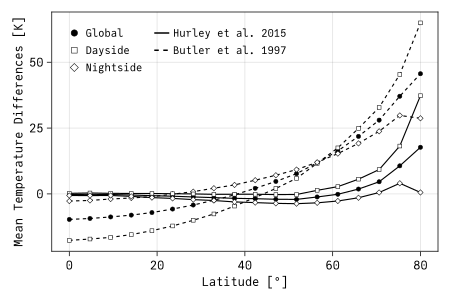
\includegraphics{moon_files/mediabag/../../img/documentation/fundamentals/planetary_bodies/moon/lunar_surface_temperatures_comparison/temperature_comparison_mean.pdf}

}

}

\subcaption{\label{fig-lunar-surface-temperatures-comparison-mean}Statistical
temperature difference mean.}
\end{minipage}%
%
\begin{minipage}[t]{0.50\linewidth}

{\centering 

\raisebox{-\height}{

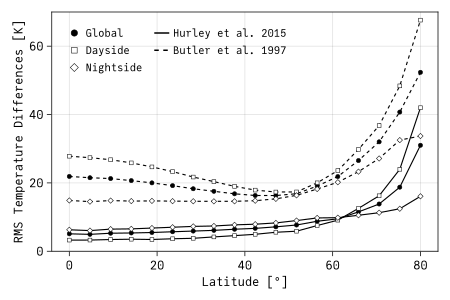
\includegraphics{moon_files/mediabag/../../img/documentation/fundamentals/planetary_bodies/moon/lunar_surface_temperatures_comparison/temperature_comparison_rms.pdf}

}

}

\subcaption{\label{fig-lunar-surface-temperatures-comparison-rms}Root
mean squared error of temperature differences.}
\end{minipage}%

\caption{\label{fig-lunar_surface_temperatures_comparison}Statistical
comparison of the lunar surface temperatures models with Diviner
measurements. Temperature difference based on analytical functions by
Butler (1997), Eq. \eqref{eq:lunar_surface_temperatures_BUTLER}, and
Hurley et al. (2015), Eq. \eqref{eq:lunar_surface_temperatures_HURLEY},
compared to the averaged Diviner measurements and evaluated on
2.7e5\,\mathrm{} grid points, equally distributed and weighted with
their respective surface area. Comparisons are represented by their
statistical mean (a) and their root mean squared error (b), applied
globally (circles), on the dayside (squares), and on the nightside
(diamonds).}

\end{figure}

\section{Julia - Mean}

\begin{Shaded}
\begin{Highlighting}[]
\ImportTok{using} \BuiltInTok{.ExESS}
\ImportTok{using} \BuiltInTok{Statistics}\NormalTok{, }\BuiltInTok{StatsBase}
\ImportTok{using} \BuiltInTok{CairoMakie}

\CommentTok{\#::. functions}
\KeywordTok{function} \FunctionTok{comparison\_rms}\NormalTok{(N}\OperatorTok{=}\FloatTok{18}\NormalTok{, name}\OperatorTok{=}\StringTok{"temperature\_comparison\_rms"}\NormalTok{)}
\NormalTok{    grid }\OperatorTok{=}\NormalTok{ ExESS.}\FunctionTok{GlobalHEALPix2DGrid}\NormalTok{(}\FloatTok{1.0}\NormalTok{,}\FloatTok{150}\NormalTok{)}

    \CommentTok{\#::. temperatures}
\NormalTok{    T\_diviner }\OperatorTok{=} \FunctionTok{lunar\_surface\_temperatures\_diviner\_avg}\NormalTok{(grid)}
\NormalTok{    T\_B }\OperatorTok{=} \FunctionTok{lunar\_surface\_temperatures\_BUTLER1997}\NormalTok{(grid)}
\NormalTok{    T\_H }\OperatorTok{=} \FunctionTok{lunar\_surface\_temperatures\_HURLEY2015}\NormalTok{(grid)}

    \CommentTok{\#::. calculate absoluate temperature differences}
\NormalTok{    dTB }\OperatorTok{=}\NormalTok{ T\_B }\OperatorTok{.{-}}\NormalTok{ T\_diviner}
\NormalTok{    dTH }\OperatorTok{=}\NormalTok{ T\_H }\OperatorTok{.{-}}\NormalTok{ T\_diviner}

    \CommentTok{\#::. error calculation}
\NormalTok{    eB, eH }\OperatorTok{=} \DataTypeTok{Float32}\NormalTok{[], }\DataTypeTok{Float32}\NormalTok{[]}
\NormalTok{    eBd, eHd }\OperatorTok{=} \DataTypeTok{Float32}\NormalTok{[], }\DataTypeTok{Float32}\NormalTok{[]}
\NormalTok{    eBn, eHn }\OperatorTok{=} \DataTypeTok{Float32}\NormalTok{[], }\DataTypeTok{Float32}\NormalTok{[]}
    \ControlFlowTok{for}\NormalTok{ i }\KeywordTok{in} \FloatTok{1}\OperatorTok{:}\NormalTok{N}
\NormalTok{        dTBlat, dTHlat }\OperatorTok{=} \DataTypeTok{Float32}\NormalTok{[], }\DataTypeTok{Float32}\NormalTok{[]}
\NormalTok{        dTBlatd, dTHlatd }\OperatorTok{=} \DataTypeTok{Float32}\NormalTok{[], }\DataTypeTok{Float32}\NormalTok{[]}
\NormalTok{        dTBlatn, dTHlatn }\OperatorTok{=} \DataTypeTok{Float32}\NormalTok{[], }\DataTypeTok{Float32}\NormalTok{[]}
        \ControlFlowTok{for}\NormalTok{ j }\KeywordTok{in} \FunctionTok{eachindex}\NormalTok{(dTB)}
            \ControlFlowTok{if}\NormalTok{ (i}\OperatorTok{{-}}\FloatTok{1}\NormalTok{)}\OperatorTok{*}\ConstantTok{pi}\OperatorTok{/}\FloatTok{2}\OperatorTok{/}\NormalTok{N }\OperatorTok{\textless{}} \FunctionTok{abs}\NormalTok{(grid.coords[j].phi) }\OperatorTok{\textless{}}\NormalTok{ i}\OperatorTok{*}\ConstantTok{pi}\OperatorTok{/}\FloatTok{2}\OperatorTok{/}\NormalTok{N; }\FunctionTok{push!}\NormalTok{(dTBlat, dTB[j]) }
                \FunctionTok{push!}\NormalTok{(dTHlat, dTH[j]) }
                \ControlFlowTok{if} \OperatorTok{{-}}\ConstantTok{pi}\OperatorTok{/}\FloatTok{2} \OperatorTok{+} \FloatTok{0.1} \OperatorTok{\textless{}}\NormalTok{ grid.coords[j].theta }\OperatorTok{\textless{}} \ConstantTok{pi}\OperatorTok{/}\FloatTok{2} \OperatorTok{{-}} \FloatTok{0.1}\NormalTok{; }\FunctionTok{push!}\NormalTok{(dTBlatd, dTB[j]); }\FunctionTok{push!}\NormalTok{(dTHlatd, dTH[j]); }\ControlFlowTok{end} \CommentTok{\# day}
                \ControlFlowTok{if}\NormalTok{ !(}\OperatorTok{{-}}\ConstantTok{pi}\OperatorTok{/}\FloatTok{2} \OperatorTok{+} \FloatTok{0.1} \OperatorTok{\textless{}}\NormalTok{ grid.coords[j].theta }\OperatorTok{\textless{}} \ConstantTok{pi}\OperatorTok{/}\FloatTok{2} \OperatorTok{{-}} \FloatTok{0.1}\NormalTok{); }\FunctionTok{push!}\NormalTok{(dTBlatn, dTB[j]); }\FunctionTok{push!}\NormalTok{(dTHlatn, dTH[j]); }\ControlFlowTok{end} \CommentTok{\# night}
            \ControlFlowTok{end}
        \ControlFlowTok{end}
        \FunctionTok{push!}\NormalTok{(eB, }\FunctionTok{sqrt}\NormalTok{(}\FunctionTok{mean}\NormalTok{(dTBlat}\OperatorTok{.\^{}}\FloatTok{2}\NormalTok{)))  }
        \FunctionTok{push!}\NormalTok{(eBd, }\FunctionTok{sqrt}\NormalTok{(}\FunctionTok{mean}\NormalTok{(dTBlatd}\OperatorTok{.\^{}}\FloatTok{2}\NormalTok{)))}
        \FunctionTok{push!}\NormalTok{(eBn, }\FunctionTok{sqrt}\NormalTok{(}\FunctionTok{mean}\NormalTok{(dTBlatn}\OperatorTok{.\^{}}\FloatTok{2}\NormalTok{)))}
        \FunctionTok{push!}\NormalTok{(eH, }\FunctionTok{sqrt}\NormalTok{(}\FunctionTok{mean}\NormalTok{(dTHlat}\OperatorTok{.\^{}}\FloatTok{2}\NormalTok{)))  }
        \FunctionTok{push!}\NormalTok{(eHd, }\FunctionTok{sqrt}\NormalTok{(}\FunctionTok{mean}\NormalTok{(dTHlatd}\OperatorTok{.\^{}}\FloatTok{2}\NormalTok{)))}
        \FunctionTok{push!}\NormalTok{(eHn, }\FunctionTok{sqrt}\NormalTok{(}\FunctionTok{mean}\NormalTok{(dTHlatn}\OperatorTok{.\^{}}\FloatTok{2}\NormalTok{)))}
    \ControlFlowTok{end}

    \CommentTok{\#::. prep figures}
\NormalTok{    fig }\OperatorTok{=} \FunctionTok{Figure}\NormalTok{(;)}
\NormalTok{    ax }\OperatorTok{=} \FunctionTok{Axis}\NormalTok{(fig[}\FloatTok{1}\NormalTok{,}\FloatTok{1}\NormalTok{];}
\NormalTok{        xlabel}\OperatorTok{=}\StringTok{"Latitude [°]"}\NormalTok{,}
\NormalTok{        xticks}\OperatorTok{=}\FloatTok{0}\OperatorTok{:}\FloatTok{20}\OperatorTok{:}\FloatTok{90}\NormalTok{,}
\NormalTok{        ylabel}\OperatorTok{=}\StringTok{"RMS Temperature Differences [K]"}\NormalTok{,}
\NormalTok{        yticks}\OperatorTok{=}\FloatTok{0}\OperatorTok{:}\FloatTok{20}\OperatorTok{:}\FloatTok{70}\NormalTok{,)}
    \FunctionTok{ylims!}\NormalTok{(}\FloatTok{0}\NormalTok{, }\FloatTok{70}\NormalTok{)}

    \CommentTok{\#::. plots}
    \FunctionTok{lines!}\NormalTok{(ax, }\FunctionTok{range}\NormalTok{(}\FloatTok{0}\NormalTok{,}\FloatTok{80}\NormalTok{,N), eB;  color}\OperatorTok{=}\NormalTok{TUMBlack, linestyle}\OperatorTok{=:}\NormalTok{dash)}
    \FunctionTok{lines!}\NormalTok{(ax, }\FunctionTok{range}\NormalTok{(}\FloatTok{0}\NormalTok{,}\FloatTok{80}\NormalTok{,N), eBd; color}\OperatorTok{=}\NormalTok{TUMBlack, linestyle}\OperatorTok{=:}\NormalTok{dash)}
    \FunctionTok{lines!}\NormalTok{(ax, }\FunctionTok{range}\NormalTok{(}\FloatTok{0}\NormalTok{,}\FloatTok{80}\NormalTok{,N), eBn; color}\OperatorTok{=}\NormalTok{TUMBlack, linestyle}\OperatorTok{=:}\NormalTok{dash)}
    \FunctionTok{lines!}\NormalTok{(ax, }\FunctionTok{range}\NormalTok{(}\FloatTok{0}\NormalTok{,}\FloatTok{80}\NormalTok{,N), eH;  color}\OperatorTok{=}\NormalTok{TUMBlack)}
    \FunctionTok{lines!}\NormalTok{(ax, }\FunctionTok{range}\NormalTok{(}\FloatTok{0}\NormalTok{,}\FloatTok{80}\NormalTok{,N), eHd; color}\OperatorTok{=}\NormalTok{TUMBlack)}
    \FunctionTok{lines!}\NormalTok{(ax, }\FunctionTok{range}\NormalTok{(}\FloatTok{0}\NormalTok{,}\FloatTok{80}\NormalTok{,N), eHn; color}\OperatorTok{=}\NormalTok{TUMBlack)}

    \FunctionTok{scatter!}\NormalTok{(ax, }\FunctionTok{range}\NormalTok{(}\FloatTok{0}\NormalTok{,}\FloatTok{80}\NormalTok{,N), eB;  color}\OperatorTok{=}\NormalTok{TUMBlack, strokecolor}\OperatorTok{=}\NormalTok{TUMBlack, strokewidth}\OperatorTok{=}\FloatTok{0.7}\NormalTok{)}
    \FunctionTok{scatter!}\NormalTok{(ax, }\FunctionTok{range}\NormalTok{(}\FloatTok{0}\NormalTok{,}\FloatTok{80}\NormalTok{,N), eBd; color}\OperatorTok{=:}\NormalTok{white, strokecolor}\OperatorTok{=}\NormalTok{TUMBlack, strokewidth}\OperatorTok{=}\FloatTok{0.7}\NormalTok{, marker}\OperatorTok{=:}\NormalTok{rect)}
    \FunctionTok{scatter!}\NormalTok{(ax, }\FunctionTok{range}\NormalTok{(}\FloatTok{0}\NormalTok{,}\FloatTok{80}\NormalTok{,N), eBn; color}\OperatorTok{=:}\NormalTok{white, strokecolor}\OperatorTok{=}\NormalTok{TUMBlack, strokewidth}\OperatorTok{=}\FloatTok{0.7}\NormalTok{, marker}\OperatorTok{=:}\NormalTok{diamond)}
    \FunctionTok{scatter!}\NormalTok{(ax, }\FunctionTok{range}\NormalTok{(}\FloatTok{0}\NormalTok{,}\FloatTok{80}\NormalTok{,N), eH;  color}\OperatorTok{=}\NormalTok{TUMBlack, strokewidth}\OperatorTok{=}\FloatTok{0.7}\NormalTok{)}
    \FunctionTok{scatter!}\NormalTok{(ax, }\FunctionTok{range}\NormalTok{(}\FloatTok{0}\NormalTok{,}\FloatTok{80}\NormalTok{,N), eHd; color}\OperatorTok{=:}\NormalTok{white, strokewidth}\OperatorTok{=}\FloatTok{0.7}\NormalTok{, marker}\OperatorTok{=:}\NormalTok{rect)}
    \FunctionTok{scatter!}\NormalTok{(ax, }\FunctionTok{range}\NormalTok{(}\FloatTok{0}\NormalTok{,}\FloatTok{80}\NormalTok{,N), eHn; color}\OperatorTok{=:}\NormalTok{white, strokewidth}\OperatorTok{=}\FloatTok{0.7}\NormalTok{, marker}\OperatorTok{=:}\NormalTok{diamond)}

    \CommentTok{\#::. legend}
\NormalTok{    l1 }\OperatorTok{=} \FunctionTok{LineElement}\NormalTok{(color}\OperatorTok{=}\NormalTok{TUMBlack, linestyle}\OperatorTok{=:}\NormalTok{dash, linewidth}\OperatorTok{=}\FloatTok{2}\NormalTok{)}
\NormalTok{    l2 }\OperatorTok{=} \FunctionTok{LineElement}\NormalTok{(color}\OperatorTok{=}\NormalTok{TUMBlack, linestyle}\OperatorTok{=:}\NormalTok{solid, linewidth}\OperatorTok{=}\FloatTok{2}\NormalTok{)}
\NormalTok{    m1 }\OperatorTok{=} \FunctionTok{MarkerElement}\NormalTok{(color}\OperatorTok{=}\NormalTok{TUMBlack, strokecolor}\OperatorTok{=}\NormalTok{TUMBlack, strokewidth}\OperatorTok{=}\FloatTok{0.7}\NormalTok{, marker}\OperatorTok{=:}\NormalTok{circle,)}
\NormalTok{    m2 }\OperatorTok{=} \FunctionTok{MarkerElement}\NormalTok{(color}\OperatorTok{=:}\NormalTok{white, strokecolor}\OperatorTok{=}\NormalTok{TUMBlack, strokewidth}\OperatorTok{=}\FloatTok{0.7}\NormalTok{, marker}\OperatorTok{=:}\NormalTok{rect,)}
\NormalTok{    m3 }\OperatorTok{=} \FunctionTok{MarkerElement}\NormalTok{(color}\OperatorTok{=:}\NormalTok{white, strokecolor}\OperatorTok{=}\NormalTok{TUMBlack, strokewidth}\OperatorTok{=}\FloatTok{0.7}\NormalTok{, marker}\OperatorTok{=:}\NormalTok{diamond,)}
    \FunctionTok{axislegend}\NormalTok{(ax,  }
\NormalTok{        [ m1, l2, m2, l1, m3],}
\NormalTok{        [ }\StringTok{"Global"}\NormalTok{, }\StringTok{"Hurley et al. 2015"}\NormalTok{, }\StringTok{"Dayside"}\NormalTok{, }\StringTok{"Butler et al. 1997"}\NormalTok{, }\StringTok{"Nightside"}\NormalTok{, ];}
\NormalTok{        position}\OperatorTok{=:}\NormalTok{lt,}
\NormalTok{        nbanks}\OperatorTok{=}\FloatTok{2}\NormalTok{,}
\NormalTok{        framevisible}\OperatorTok{=}\ConstantTok{false}\NormalTok{,}
\NormalTok{    )}

    \CommentTok{\#::. save figure}
    \FunctionTok{save}\NormalTok{(}\FunctionTok{joinpath}\NormalTok{(}\PreprocessorTok{@\_\_DIR\_\_}\NormalTok{, }\StringTok{"}\SpecialCharTok{$}\NormalTok{(name)}\StringTok{.pdf"}\NormalTok{), fig)}
    \FunctionTok{save}\NormalTok{(}\FunctionTok{joinpath}\NormalTok{(}\PreprocessorTok{@\_\_DIR\_\_}\NormalTok{, }\StringTok{"}\SpecialCharTok{$}\NormalTok{(name)}\StringTok{.svg"}\NormalTok{), fig)}
    \FunctionTok{save}\NormalTok{(}\FunctionTok{joinpath}\NormalTok{(}\PreprocessorTok{@\_\_DIR\_\_}\NormalTok{, }\StringTok{"}\SpecialCharTok{$}\NormalTok{(name)}\StringTok{.png"}\NormalTok{), fig, px\_per\_unit}\OperatorTok{=}\FloatTok{4}\NormalTok{)}

    \ControlFlowTok{return} \ConstantTok{nothing}
\KeywordTok{end}
\end{Highlighting}
\end{Shaded}

\section{Julia - RMS}

\begin{Shaded}
\begin{Highlighting}[]
\ImportTok{using} \BuiltInTok{.ExESS}
\ImportTok{using} \BuiltInTok{Statistics}\NormalTok{, }\BuiltInTok{StatsBase}
\ImportTok{using} \BuiltInTok{CairoMakie}

\CommentTok{\#::. functions}
\KeywordTok{function} \FunctionTok{comparison\_mean}\NormalTok{(N}\OperatorTok{=}\FloatTok{18}\NormalTok{, name}\OperatorTok{=}\StringTok{"temperature\_comparison\_mean"}\NormalTok{)}
\NormalTok{    grid }\OperatorTok{=}\NormalTok{ ExESS.}\FunctionTok{GlobalHEALPix2DGrid}\NormalTok{(}\FloatTok{1.0}\NormalTok{,}\FloatTok{150}\NormalTok{)}

    \CommentTok{\#::. temperatures}
\NormalTok{    T\_diviner }\OperatorTok{=} \FunctionTok{lunar\_surface\_temperatures\_diviner\_avg}\NormalTok{(grid)}
\NormalTok{    T\_B }\OperatorTok{=} \FunctionTok{lunar\_surface\_temperatures\_BUTLER1997}\NormalTok{(grid)}
\NormalTok{    T\_H }\OperatorTok{=} \FunctionTok{lunar\_surface\_temperatures\_HURLEY2015}\NormalTok{(grid)}

    \CommentTok{\#::. calculate absoluate temperature differences}
\NormalTok{    dTB }\OperatorTok{=}\NormalTok{ T\_B }\OperatorTok{.{-}}\NormalTok{ T\_diviner}
\NormalTok{    dTH }\OperatorTok{=}\NormalTok{ T\_H }\OperatorTok{.{-}}\NormalTok{ T\_diviner}

    \CommentTok{\#::. error calculation}
\NormalTok{    eB, eH }\OperatorTok{=} \DataTypeTok{Float32}\NormalTok{[], }\DataTypeTok{Float32}\NormalTok{[]}
\NormalTok{    eBd, eHd }\OperatorTok{=} \DataTypeTok{Float32}\NormalTok{[], }\DataTypeTok{Float32}\NormalTok{[]}
\NormalTok{    eBn, eHn }\OperatorTok{=} \DataTypeTok{Float32}\NormalTok{[], }\DataTypeTok{Float32}\NormalTok{[]}
    \ControlFlowTok{for}\NormalTok{ i }\KeywordTok{in} \FloatTok{1}\OperatorTok{:}\NormalTok{N}
\NormalTok{        dTBlat, dTHlat }\OperatorTok{=} \DataTypeTok{Float32}\NormalTok{[], }\DataTypeTok{Float32}\NormalTok{[]}
\NormalTok{        dTBlatd, dTHlatd }\OperatorTok{=} \DataTypeTok{Float32}\NormalTok{[], }\DataTypeTok{Float32}\NormalTok{[]}
\NormalTok{        dTBlatn, dTHlatn }\OperatorTok{=} \DataTypeTok{Float32}\NormalTok{[], }\DataTypeTok{Float32}\NormalTok{[]}
        \ControlFlowTok{for}\NormalTok{ j }\KeywordTok{in} \FunctionTok{eachindex}\NormalTok{(dTB)}
            \ControlFlowTok{if}\NormalTok{ (i}\OperatorTok{{-}}\FloatTok{1}\NormalTok{)}\OperatorTok{*}\ConstantTok{pi}\OperatorTok{/}\FloatTok{2}\OperatorTok{/}\NormalTok{N }\OperatorTok{\textless{}} \FunctionTok{abs}\NormalTok{(grid.coords[j].phi) }\OperatorTok{\textless{}}\NormalTok{ i}\OperatorTok{*}\ConstantTok{pi}\OperatorTok{/}\FloatTok{2}\OperatorTok{/}\NormalTok{N; }\FunctionTok{push!}\NormalTok{(dTBlat, dTB[j]) }
                \FunctionTok{push!}\NormalTok{(dTHlat, dTH[j]) }
                \ControlFlowTok{if} \OperatorTok{{-}}\ConstantTok{pi}\OperatorTok{/}\FloatTok{2} \OperatorTok{+} \FloatTok{0.1} \OperatorTok{\textless{}}\NormalTok{ grid.coords[j].theta }\OperatorTok{\textless{}} \ConstantTok{pi}\OperatorTok{/}\FloatTok{2} \OperatorTok{{-}} \FloatTok{0.1}\NormalTok{; }\FunctionTok{push!}\NormalTok{(dTBlatd, dTB[j]); }\FunctionTok{push!}\NormalTok{(dTHlatd, dTH[j]); }\ControlFlowTok{end} \CommentTok{\# day}
                \ControlFlowTok{if}\NormalTok{ !(}\OperatorTok{{-}}\ConstantTok{pi}\OperatorTok{/}\FloatTok{2} \OperatorTok{+} \FloatTok{0.1} \OperatorTok{\textless{}}\NormalTok{ grid.coords[j].theta }\OperatorTok{\textless{}} \ConstantTok{pi}\OperatorTok{/}\FloatTok{2} \OperatorTok{{-}} \FloatTok{0.1}\NormalTok{); }\FunctionTok{push!}\NormalTok{(dTBlatn, dTB[j]); }\FunctionTok{push!}\NormalTok{(dTHlatn, dTH[j]); }\ControlFlowTok{end} \CommentTok{\# night}
            \ControlFlowTok{end}
        \ControlFlowTok{end}
        \FunctionTok{push!}\NormalTok{(eB, }\FunctionTok{mean}\NormalTok{(dTBlat))   }
        \FunctionTok{push!}\NormalTok{(eBd, }\FunctionTok{mean}\NormalTok{(dTBlatd)) }
        \FunctionTok{push!}\NormalTok{(eBn, }\FunctionTok{mean}\NormalTok{(dTBlatn)) }
        \FunctionTok{push!}\NormalTok{(eH, }\FunctionTok{mean}\NormalTok{(dTHlat))   }
        \FunctionTok{push!}\NormalTok{(eHd, }\FunctionTok{mean}\NormalTok{(dTHlatd)) }
        \FunctionTok{push!}\NormalTok{(eHn, }\FunctionTok{mean}\NormalTok{(dTHlatn)) }
    \ControlFlowTok{end}

    \CommentTok{\#::. prep figures}
\NormalTok{    fig }\OperatorTok{=} \FunctionTok{Figure}\NormalTok{(;)}
\NormalTok{    ax }\OperatorTok{=} \FunctionTok{Axis}\NormalTok{(fig[}\FloatTok{1}\NormalTok{,}\FloatTok{1}\NormalTok{];}
\NormalTok{        xlabel}\OperatorTok{=}\StringTok{"Latitude [°]"}\NormalTok{,}
\NormalTok{        xticks}\OperatorTok{=}\FloatTok{0}\OperatorTok{:}\FloatTok{20}\OperatorTok{:}\FloatTok{90}\NormalTok{,}
\NormalTok{        ylabel}\OperatorTok{=}\StringTok{"Mean Temperature Differences [K]"}\NormalTok{)}

    \CommentTok{\#::. plots}
    \FunctionTok{lines!}\NormalTok{(ax, }\FunctionTok{range}\NormalTok{(}\FloatTok{0}\NormalTok{,}\FloatTok{80}\NormalTok{,N), eB;  color}\OperatorTok{=}\NormalTok{TUMBlack, linestyle}\OperatorTok{=:}\NormalTok{dash, )}
    \FunctionTok{lines!}\NormalTok{(ax, }\FunctionTok{range}\NormalTok{(}\FloatTok{0}\NormalTok{,}\FloatTok{80}\NormalTok{,N), eBd; color}\OperatorTok{=}\NormalTok{TUMBlack, linestyle}\OperatorTok{=:}\NormalTok{dash, )}
    \FunctionTok{lines!}\NormalTok{(ax, }\FunctionTok{range}\NormalTok{(}\FloatTok{0}\NormalTok{,}\FloatTok{80}\NormalTok{,N), eBn; color}\OperatorTok{=}\NormalTok{TUMBlack, linestyle}\OperatorTok{=:}\NormalTok{dash, )}
    \FunctionTok{lines!}\NormalTok{(ax, }\FunctionTok{range}\NormalTok{(}\FloatTok{0}\NormalTok{,}\FloatTok{80}\NormalTok{,N), eH;  color}\OperatorTok{=}\NormalTok{TUMBlack)}
    \FunctionTok{lines!}\NormalTok{(ax, }\FunctionTok{range}\NormalTok{(}\FloatTok{0}\NormalTok{,}\FloatTok{80}\NormalTok{,N), eHd; color}\OperatorTok{=}\NormalTok{TUMBlack)}
    \FunctionTok{lines!}\NormalTok{(ax, }\FunctionTok{range}\NormalTok{(}\FloatTok{0}\NormalTok{,}\FloatTok{80}\NormalTok{,N), eHn; color}\OperatorTok{=}\NormalTok{TUMBlack)}

    \FunctionTok{scatter!}\NormalTok{(ax, }\FunctionTok{range}\NormalTok{(}\FloatTok{0}\NormalTok{,}\FloatTok{80}\NormalTok{,N), eB;  color}\OperatorTok{=}\NormalTok{TUMBlack, strokecolor}\OperatorTok{=}\NormalTok{TUMBlack, strokewidth}\OperatorTok{=}\FloatTok{0.7}\NormalTok{)}
    \FunctionTok{scatter!}\NormalTok{(ax, }\FunctionTok{range}\NormalTok{(}\FloatTok{0}\NormalTok{,}\FloatTok{80}\NormalTok{,N), eBd; color}\OperatorTok{=:}\NormalTok{white, strokecolor}\OperatorTok{=}\NormalTok{TUMBlack, strokewidth}\OperatorTok{=}\FloatTok{0.7}\NormalTok{, marker}\OperatorTok{=:}\NormalTok{rect)}
    \FunctionTok{scatter!}\NormalTok{(ax, }\FunctionTok{range}\NormalTok{(}\FloatTok{0}\NormalTok{,}\FloatTok{80}\NormalTok{,N), eBn; color}\OperatorTok{=:}\NormalTok{white, strokecolor}\OperatorTok{=}\NormalTok{TUMBlack, strokewidth}\OperatorTok{=}\FloatTok{0.7}\NormalTok{, marker}\OperatorTok{=:}\NormalTok{diamond)}
    \FunctionTok{scatter!}\NormalTok{(ax, }\FunctionTok{range}\NormalTok{(}\FloatTok{0}\NormalTok{,}\FloatTok{80}\NormalTok{,N), eH;  color}\OperatorTok{=}\NormalTok{TUMBlack, strokewidth}\OperatorTok{=}\FloatTok{0.7}\NormalTok{)}
    \FunctionTok{scatter!}\NormalTok{(ax, }\FunctionTok{range}\NormalTok{(}\FloatTok{0}\NormalTok{,}\FloatTok{80}\NormalTok{,N), eHd; color}\OperatorTok{=:}\NormalTok{white, strokewidth}\OperatorTok{=}\FloatTok{0.7}\NormalTok{, marker}\OperatorTok{=:}\NormalTok{rect)}
    \FunctionTok{scatter!}\NormalTok{(ax, }\FunctionTok{range}\NormalTok{(}\FloatTok{0}\NormalTok{,}\FloatTok{80}\NormalTok{,N), eHn; color}\OperatorTok{=:}\NormalTok{white, strokewidth}\OperatorTok{=}\FloatTok{0.7}\NormalTok{, marker}\OperatorTok{=:}\NormalTok{diamond)}

    \CommentTok{\#::. legend}
\NormalTok{    l1 }\OperatorTok{=} \FunctionTok{LineElement}\NormalTok{(color}\OperatorTok{=}\NormalTok{TUMBlack, linestyle}\OperatorTok{=:}\NormalTok{dash, linewidth}\OperatorTok{=}\FloatTok{2}\NormalTok{)}
\NormalTok{    l2 }\OperatorTok{=} \FunctionTok{LineElement}\NormalTok{(color}\OperatorTok{=}\NormalTok{TUMBlack, linestyle}\OperatorTok{=:}\NormalTok{solid, linewidth}\OperatorTok{=}\FloatTok{2}\NormalTok{)}
\NormalTok{    m1 }\OperatorTok{=} \FunctionTok{MarkerElement}\NormalTok{(color}\OperatorTok{=}\NormalTok{TUMBlack, strokecolor}\OperatorTok{=}\NormalTok{TUMBlack, strokewidth}\OperatorTok{=}\FloatTok{0.7}\NormalTok{, marker}\OperatorTok{=:}\NormalTok{circle,)}
\NormalTok{    m2 }\OperatorTok{=} \FunctionTok{MarkerElement}\NormalTok{(color}\OperatorTok{=:}\NormalTok{white, strokecolor}\OperatorTok{=}\NormalTok{TUMBlack, strokewidth}\OperatorTok{=}\FloatTok{0.7}\NormalTok{, marker}\OperatorTok{=:}\NormalTok{rect,)}
\NormalTok{    m3 }\OperatorTok{=} \FunctionTok{MarkerElement}\NormalTok{(color}\OperatorTok{=:}\NormalTok{white, strokecolor}\OperatorTok{=}\NormalTok{TUMBlack, strokewidth}\OperatorTok{=}\FloatTok{0.7}\NormalTok{, marker}\OperatorTok{=:}\NormalTok{diamond,)}
    \FunctionTok{axislegend}\NormalTok{(ax,  }
\NormalTok{    [ m1, l2, m2, l1, m3],}
\NormalTok{        [ }\StringTok{"Global"}\NormalTok{, }\StringTok{"Hurley et al. 2015"}\NormalTok{, }\StringTok{"Dayside"}\NormalTok{, }\StringTok{"Butler et al. 1997"}\NormalTok{, }\StringTok{"Nightside"}\NormalTok{, ];}
\NormalTok{        position}\OperatorTok{=:}\NormalTok{lt,}
\NormalTok{        nbanks}\OperatorTok{=}\FloatTok{2}\NormalTok{,}
\NormalTok{        framevisible}\OperatorTok{=}\ConstantTok{false}
\NormalTok{    )}

    \CommentTok{\#::. save figure}
    \FunctionTok{save}\NormalTok{(}\FunctionTok{joinpath}\NormalTok{(}\PreprocessorTok{@\_\_DIR\_\_}\NormalTok{, }\StringTok{"}\SpecialCharTok{$}\NormalTok{(name)}\StringTok{.pdf"}\NormalTok{), fig)}
    \FunctionTok{save}\NormalTok{(}\FunctionTok{joinpath}\NormalTok{(}\PreprocessorTok{@\_\_DIR\_\_}\NormalTok{, }\StringTok{"}\SpecialCharTok{$}\NormalTok{(name)}\StringTok{.svg"}\NormalTok{), fig)}
    \FunctionTok{save}\NormalTok{(}\FunctionTok{joinpath}\NormalTok{(}\PreprocessorTok{@\_\_DIR\_\_}\NormalTok{, }\StringTok{"}\SpecialCharTok{$}\NormalTok{(name)}\StringTok{.png"}\NormalTok{), fig, px\_per\_unit}\OperatorTok{=}\FloatTok{4}\NormalTok{)}

    \ControlFlowTok{return} \ConstantTok{nothing}
\KeywordTok{end}
\end{Highlighting}
\end{Shaded}

\section{Downloads}

\begin{itemize}
\item
\item
\end{itemize}

\input{src/temperatures/figures/lunar_surface_temperatures_comparison.tex}

The two presented analytical models of the lunar surface temperatures
have been compared with the averaged \(\mathrm{DLRE}\) measurements.
Figure~\ref{fig-lunar_surface_temperatures_comparison} shows this
statistical analysis of the temperatures difference of the Butler (1997)
and Hurley et al. (2015) calculated as
\(\Delta T_i = T_i - T_\text{Diviner}\) for each analytical model \(i\),
evaluated on 270e3\,\mathrm{} surface points, globally distributed using
the \href{/documentation/math_num_comp/numerical_grids.qmd}{HEALPix}
method.

The left side shows the statistical mean of said temperature differences
as a function of subsolar latitude for both models, both globally as
well as exclusively on the dayside and nightside of the Moon. Up to
\(\Phi_{ss}=60\,\mathrm{\degree}\), the Hurley et al. (2015) model has
global means very close to zero, with slight deviations for the
exclusive day- and nightside. Closer to the poles, the model tends
towards positive temperature differences, peaking at around
35\,\mathrm{K} above the Diviner model on the sunlit side. Using the
model by Butler (1997) this effect is even more pronounced with the
means starting below zero at the equator and continuously increasing
with higher latitudes. Final values close to the poles reach temperature
differences of more than 60\,\mathrm{K} on the dayside.

To further investigate the two models, the \(\mathrm{rms}\) value of the
temperature differences \begin{equation}
    \Delta T_{\text{rms}, i} = \sqrt{\frac{1}{N_j} \cdot \sum_j^{N_j} \left(\Delta T_{i,j}\right)^2},
\end{equation} for \(N_j\) applicable positions \(j\) is shown on the
right side of Figure~\ref{fig-lunar_surface_temperatures_comparison}. In
comparison with the previously shown statistical mean, the
\(\mathrm{rms}\) shows the spread of the temperatures around the mean.
For all cases, globally, dayside, and nightside, the Hurley et al.
(2015) model has lower \(\mathrm{rms}\) values, which are less than
10\,\mathrm{K} for latitude uo to 60\,\mathrm{\degree}. Closer to the
poles and similar to the mean value, the dayside temperatures tend to
deviate the most, peaking at 43\,\mathrm{K} at 80\,\mathrm{\degree}.
Generally, a steadily increasing behaviour with higher latitudes can be
observed. For the Butler (1997) model, the \(\mathrm{rms}\) values start
out considerably higher with the worst deviations on the dayside of the
Moon. For roughly 50\,\mathrm{\degree} from the equator, the values are
decreasing to a lowest value of 17\,\mathrm{K} before sharply increasing
polewards of it.

\hypertarget{ref}{}

\hypertarget{refs}{}
\begin{CSLReferences}{1}{0}
\leavevmode\vadjust pre{\hypertarget{ref-Butler1997}{}}%
Butler, Bryan J. 1997. {``The Migration of Volatiles on the Surfaces of
{M}ercury and the {M}oon.''} \emph{Journal of Geophysical Research} 102
(E8): 19, 283--19, 291. \url{https://doi.org/10.1029/97JE01347}.

\leavevmode\vadjust pre{\hypertarget{ref-Hurley2015}{}}%
Hurley, Dana M., Menelaos Sarantos, Cesare Grava, Jean-Pierre Williams,
Kurt D. Retherford, Matthew Siegler, Benjamin Greenhagen, and David
Paige. 2015. {``An Analytic Function of Lunar Surface Temperature for
Exospheric Modeling.''} \emph{Icarus} 255 (July): 159--63.
\url{https://doi.org/10.1016/j.icarus.2014.08.043}.

\leavevmode\vadjust pre{\hypertarget{ref-Vasavada2012}{}}%
Vasavada, Ashwin R., Joshua L. Bandfield, Benjamin T. Greenhagen, Paul
O. Hayne, Matthew A. Siegler, Jean-Pierre Williams, and David A. Paige.
2012. {``{Lunar equatorial surface temperatures and regolith properties
from the Diviner lunar radiometer experiment}.''}
\url{https://doi.org/10.1029/2011JE003987}.

\end{CSLReferences}
\end{document}
